\begin{figure}[h!]
	\centering
	
	
	\tikzset{every picture/.style={line width=0.75pt}} %set default line width to 0.75pt        
	
	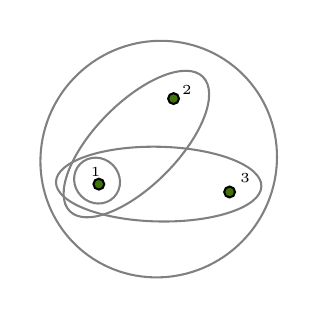
\begin{tikzpicture}[x=0.75pt,y=0.75pt,yscale=-0.9,xscale=0.9]
		%uncomment if require: \path (0,300); %set diagram left start at 0, and has height of 300
		
		%Shape: Circle [id:dp6254924747106434] 
		\draw  [fill={rgb, 255:red, 65; green, 117; blue, 5 }  ,fill opacity=1 ] (180,132.9) .. controls (180,131.3) and (181.3,130) .. (182.9,130) .. controls (184.5,130) and (185.8,131.3) .. (185.8,132.9) .. controls (185.8,134.5) and (184.5,135.8) .. (182.9,135.8) .. controls (181.3,135.8) and (180,134.5) .. (180,132.9) -- cycle ;
		%Shape: Circle [id:dp48431322085787665] 
		\draw  [fill={rgb, 255:red, 65; green, 117; blue, 5 }  ,fill opacity=1 ] (250,137.1) .. controls (250,135.5) and (251.3,134.2) .. (252.9,134.2) .. controls (254.5,134.2) and (255.8,135.5) .. (255.8,137.1) .. controls (255.8,138.7) and (254.5,140) .. (252.9,140) .. controls (251.3,140) and (250,138.7) .. (250,137.1) -- cycle ;
		%Shape: Circle [id:dp35320390948185487] 
		\draw  [fill={rgb, 255:red, 65; green, 117; blue, 5 }  ,fill opacity=1 ] (220,87.1) .. controls (220,85.5) and (221.3,84.2) .. (222.9,84.2) .. controls (224.5,84.2) and (225.8,85.5) .. (225.8,87.1) .. controls (225.8,88.7) and (224.5,90) .. (222.9,90) .. controls (221.3,90) and (220,88.7) .. (220,87.1) -- cycle ;
		%Shape: Ellipse [id:dp6827777295590995] 
		\draw  [color={rgb, 255:red, 128; green, 128; blue, 128 }  ,draw opacity=1 ] (167.37,147.4) .. controls (158.67,138.78) and (167.57,115.69) .. (187.24,95.83) .. controls (206.91,75.96) and (229.91,66.84) .. (238.61,75.46) .. controls (247.3,84.07) and (238.41,107.16) .. (218.74,127.02) .. controls (199.07,146.89) and (176.07,156.01) .. (167.37,147.4) -- cycle ;
		%Shape: Ellipse [id:dp2922418509608795] 
		\draw  [color={rgb, 255:red, 128; green, 128; blue, 128 }  ,draw opacity=1 ] (159.96,131.71) .. controls (160.2,120.67) and (185,112.24) .. (215.36,112.88) .. controls (245.73,113.53) and (270.15,123.01) .. (269.91,134.05) .. controls (269.68,145.09) and (244.87,153.52) .. (214.51,152.87) .. controls (184.15,152.23) and (159.73,142.75) .. (159.96,131.71) -- cycle ;
		%Shape: Ellipse [id:dp2556128273268483] 
		\draw  [color={rgb, 255:red, 128; green, 128; blue, 128 }  ,draw opacity=1 ] (173.59,139.43) .. controls (168.61,134.5) and (168.32,126.73) .. (172.93,122.07) .. controls (177.55,117.41) and (185.32,117.63) .. (190.3,122.55) .. controls (195.28,127.48) and (195.57,135.26) .. (190.96,139.92) .. controls (186.34,144.58) and (178.57,144.36) .. (173.59,139.43) -- cycle ;
		%Shape: Ellipse [id:dp36749477614063886] 
		\draw  [color={rgb, 255:red, 128; green, 128; blue, 128 }  ,draw opacity=1 ] (169.98,164.9) .. controls (145.36,140.52) and (145.53,100.42) .. (170.37,75.34) .. controls (195.21,50.26) and (235.3,49.69) .. (259.92,74.07) .. controls (284.54,98.45) and (284.36,138.55) .. (259.53,163.63) .. controls (234.69,188.71) and (194.6,189.28) .. (169.98,164.9) -- cycle ;
		
		% Text Node
		\draw (177,122.4) node [anchor=north west][inner sep=0.75pt]  [font=\tiny]  {$1$};
		% Text Node
		\draw (225.8,78.4) node [anchor=north west][inner sep=0.75pt]  [font=\tiny]  {$2$};
		% Text Node
		\draw (257,125.6) node [anchor=north west][inner sep=0.75pt]  [font=\tiny]  {$3$};
		
		
	\end{tikzpicture}
\end{figure}